\documentclass[11pt]{beamer}
\usepackage{xeCJK}
\setCJKmainfont{蘋方-繁}
\renewcommand{\baselinestretch}{1.5}
\usepackage[T1]{fontenc}
\usetheme{CambridgeUS}
\usepackage[osf]{MinionPro}
\usepackage{MyriadPro}
\usecolortheme{beaver}

\newcommand*{\dif}{\,\mathrm{d}}
\newtheorem*{definition*}{Definition}
\newtheorem*{corollary*}{Corollary}
\def\tb#1#2{\mathop{#1\vphantom{\sum}}\limits_{\displaystyle #2}}
\usefonttheme{professionalfonts}

\usepackage{amsmath, amssymb, amsthm}
\newtheorem{prop}{\scshape Proposition}
\newenvironment{propc}[1]
{\begin{prop}}
        {\end{prop}}
\setbeamertemplate{theorems}[numbered]

\AtBeginSection[]{
  \begin{frame}
  \vfill
  \centering
  \begin{beamercolorbox}[sep=8pt,center,shadow=true,rounded=true]{title}
    \usebeamerfont{title}\insertsectionhead\par%
  \end{beamercolorbox}
  \vfill
  \end{frame}
}

\usepackage{tikz}
\usepackage{booktabs,tabulary}
\usepackage{threeparttable}

\title{The Second Hand Market of iPhone in PTT Macshop Board}
\author{陳柏瑜, 高翊傑}
\institute[NTU Econ]{\scshape 109-1 ECON-DSSI\\ NTU ECON}
\date{2021.1.4}

\begin{document}
\begin{frame}
\titlepage
\end{frame}

\begin{frame}
\frametitle{Outline}
\tableofcontents
\end{frame}


\section{Core Question}

	\begin{enumerate}
		\item 「女用機」比較值錢?
		\item Estimating the second-hand iPhone Demand
		\item The probability of successfully selling an iPhone 6s
		\item Analysis based on the geographical distribution of second hand iPhone selling and buying
	\end{enumerate}

\section{Data Description} 

\section{Descriptive Statistics} 

\section{Results}


\subsection{「女用機」比較值錢?}
%%%
\begin{frame}[fragile]{「女用機」比較值錢?}

	\begin{itemize}
		\item 欲出售 iphone 的貼文內標注「女用機」或「女生用」
		\item 「女用機」真的可以賣得比較貴嗎?
		\item 將此 “premium” 稱為 “gender rent”
	\end{itemize}


\end{frame}


%%%
\begin{frame}[fragile]{「女用機」比較值錢?}

在 163950 則交易iPhone的貼文

	\begin{itemize}
		\item 標注「男用機」: 83 則;標注「女用機」: 2922 則
		\item 需要區別「成交價格」以及「非成交價格」
	\end{itemize}

考量線性迴歸模型:

$$price_i = \beta_0 + \beta_1 D_{female, i} + \beta_2 D_{male, i} + \gamma W_i + u_i$$

where $W$ is the control variable and $W$ contains: $$TimeUsed, ROM, color$$

\end{frame}


%%%
\begin{frame}[fragile]{「女用機」比較值錢?}

	\begin{figure}
		\begin{center}
			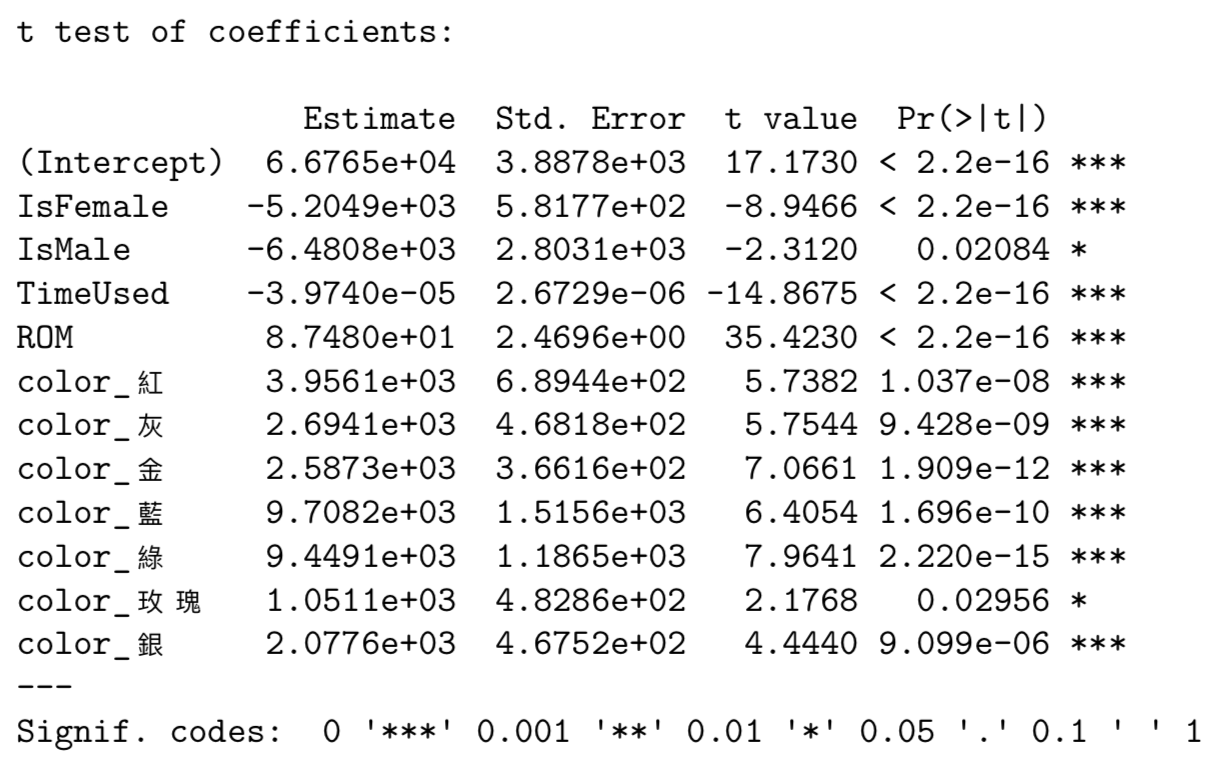
\includegraphics[width=0.8\textwidth]{figure/f01.png}
		\end{center}
	\end{figure}

\end{frame}


%%%
\begin{frame}[fragile]{「女用機」比較值錢?}

	\begin{itemize}
		\item 與預期相反,在所有型號中且是「已售出」或「已徵得」的 iPhone 中,標注有「女用機」的貼文的成交價格是比較低的。
		\item 若是限制在 iPhone 6s 這個機型的話,則沒有顯著地異於零,但大致的方向仍是負的,意味著標示「女用機」並沒有辦法「提升價格」。
		\item 在 PTT 的文化中,更常見的是嘲諷標注女用機的貼文者
	\end{itemize}

\end{frame}


%%%
\begin{frame}[fragile]{「女用機」比較值錢?}

考量線性迴歸模型,並將樣本限制在成交的iPhone 6s貼文中:
$$price_i = \beta_0 + \beta_1 D_{female, i} + \beta_2 D_{male, i} + \gamma W_i + u_i$$
where $W$ is the control variable and $W$ contains: $$TimeUsed, ROM, color$$

\end{frame}


%%%
\begin{frame}[fragile]{「女用機」比較值錢?}

	\begin{figure}
		\begin{center}
			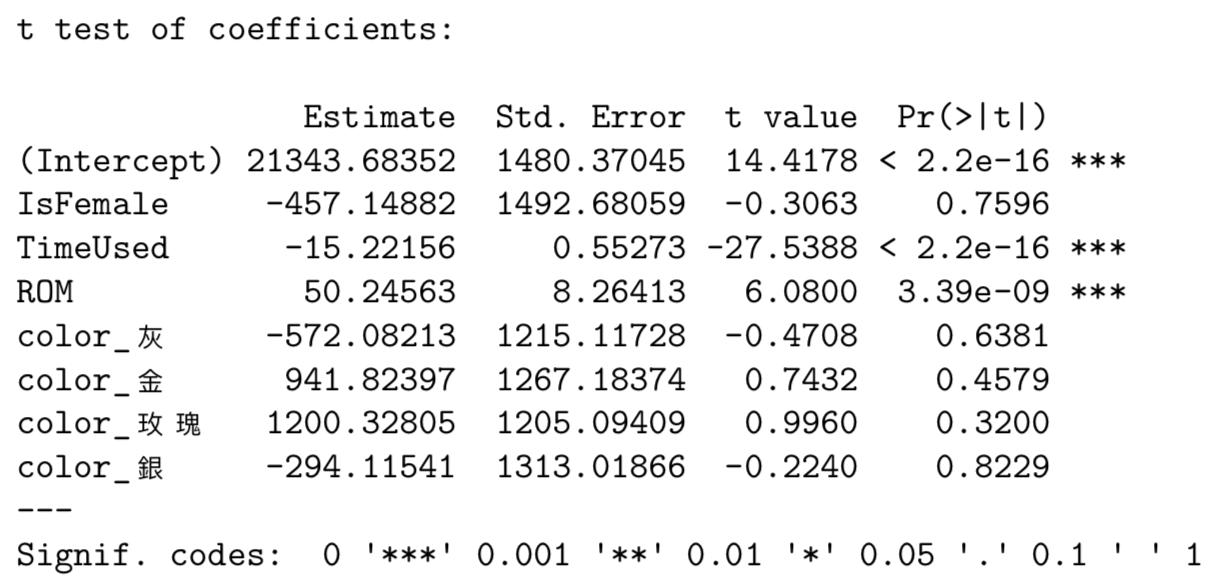
\includegraphics[width=0.8\textwidth]{figure/f02.png}
		\end{center}
	\end{figure}

\end{frame}


\subsection{Estimating the second-hand iPhone Demand}

%%%
\begin{frame}[fragile]{Definition}

	\begin{itemize}
		\item Demand function characterizes the quantity demanded $q^d$ when given a price $p$
	\end{itemize}
	Notice that $q^d$ is a function of $p$

	\begin{itemize}
		\item The Inverse Demand function characterizes the price $p$ when given a quantity demanded $q^d$
		\item Economists usually use inverse demand to characterize the "Willingness to Pay"
	\end{itemize}

\end{frame}


%%%
\begin{frame}[fragile]{Definition}

	\begin{figure}
		\begin{center}
			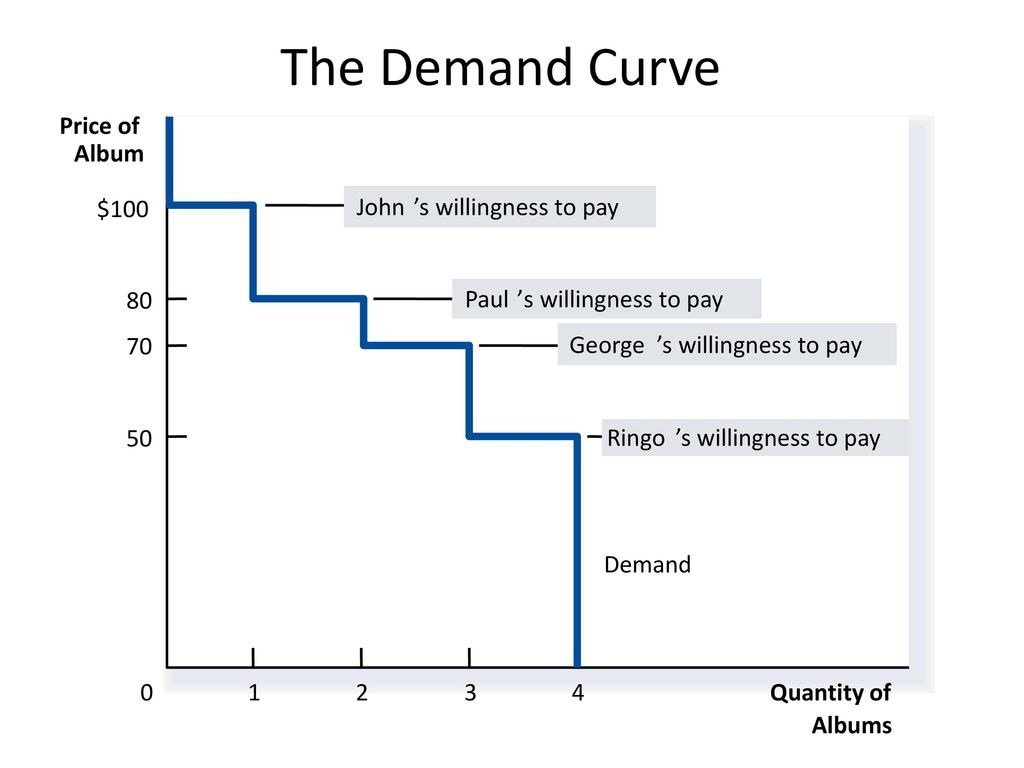
\includegraphics[width=0.8\textwidth]{figure/f03.png}
		\end{center}
	\end{figure}

\end{frame}


%%%
\begin{frame}[fragile]{Estimating Demand?}

If we do not restrict the data on the SOLD and BOUGHT one, then we are not at the equilibrium.
	\begin{itemize}
		\item If we do not restrict the data on the SOLD and BOUGHT one, then we are not at the equilibrium.
		\item However, we have the label: Whether the poster is a potential buyer or seller.
		\item Thus, we're looking the Willingness to pay (WTP) for buyers.
		\item What about sellers? "Willingness to be paid" (WTBP)
	\end{itemize}
\end{frame}

%%%
\begin{frame}[fragile]{Estimating WTP and WTBP}

由於 iPhone 6s 此一機型非常地暢銷,自 2015 年發售以來便持續活躍於二手交易市場,以致於在關鍵字為 iPhone 的 19 萬則貼文中,儘 管 iPhone 有從 3GS 到 iPhone 12 等數十個型號,但仍有近 10\% 的貼文是此單一機型,因此我們將所估計的財貨限制在此一型號

由於二手交易版需要使用者在貼文時標注自己希望「出售」還是「購買」(徵求)。在使用者打算「徵求」購買一支二手的手機時,我們可以將帶
有「購買」分類標籤的貼文簡單地視為使用者標注了自己的 “Willingness To Pay”(願付價格);而對於打算出售二手手機的使用者,文內的 「希望價格」我們則以 “Willingness To Be Paid” 來稱之。


\end{frame}

%%%
\begin{frame}[fragile]{Estimating WTP and WTBP}

若分別以 inverse supply function 以及 inverse demand function 的角度視之,我們可以分別寫下:
$$ p_t = \alpha_0 + \alpha_1 q_t^s + \alpha W_t + u_t$$
$$ p_t = \beta_0 + \beta_1 q_t^s + \beta W_t + v_t$$
where $q_t^s, q_t^d$ 分別代表時間$t$時,iPhone 6s 的供給以及需求

\end{frame}


%%%
\begin{frame}[fragile]{Estimating WTP and WTBP}

在此,由於我們有區別是在 supply side 或 demand side 的分類標籤,因此無須處理 simultaneous equation 的問題。當然,我們 所估計的上面兩條迴歸式尚且不能稱之為供給及需求函數,但可以作為此二函數的近似。在此,我們尚且稱呼此二式為 Willingness To Be Paid (WTBP) 及 Willingness To Pay (WTP)

\end{frame}


%%%
\begin{frame}[fragile]{Estimating WTBP}

WTBP:
$$p = 22346.26 + 20.54 q^s$$

	\begin{figure}
		\begin{center}
			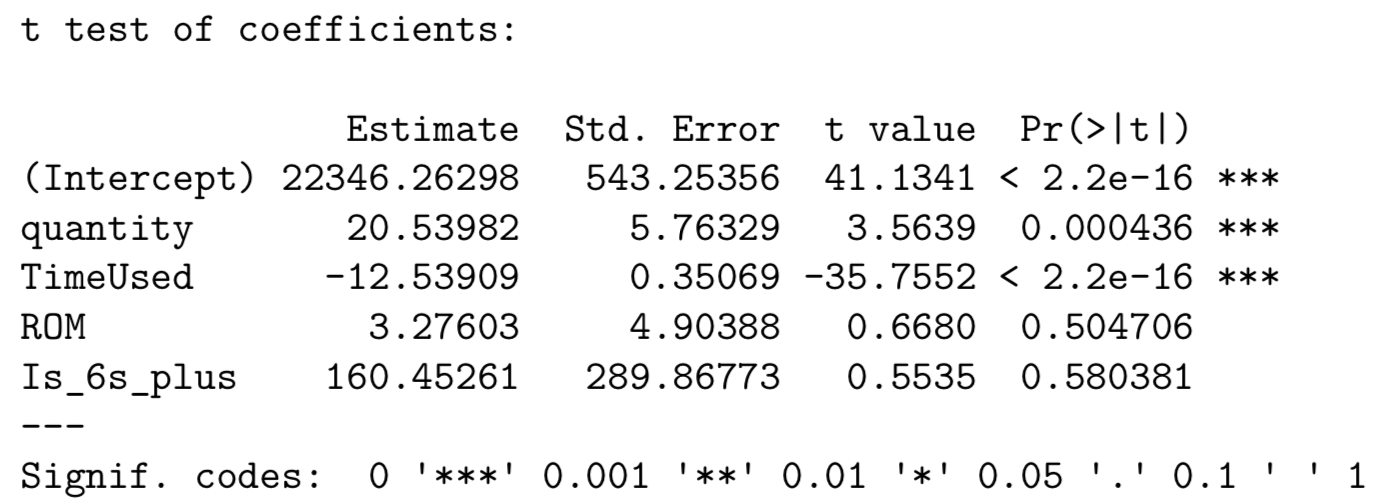
\includegraphics[width=0.8\textwidth]{figure/f04.png}
		\end{center}
	\end{figure}

\end{frame}

%%%
\begin{frame}[fragile]{Estimating WTP}

WTBP:
$$p = 23691.78 - 8.54 q^d$$

	\begin{figure}
		\begin{center}
			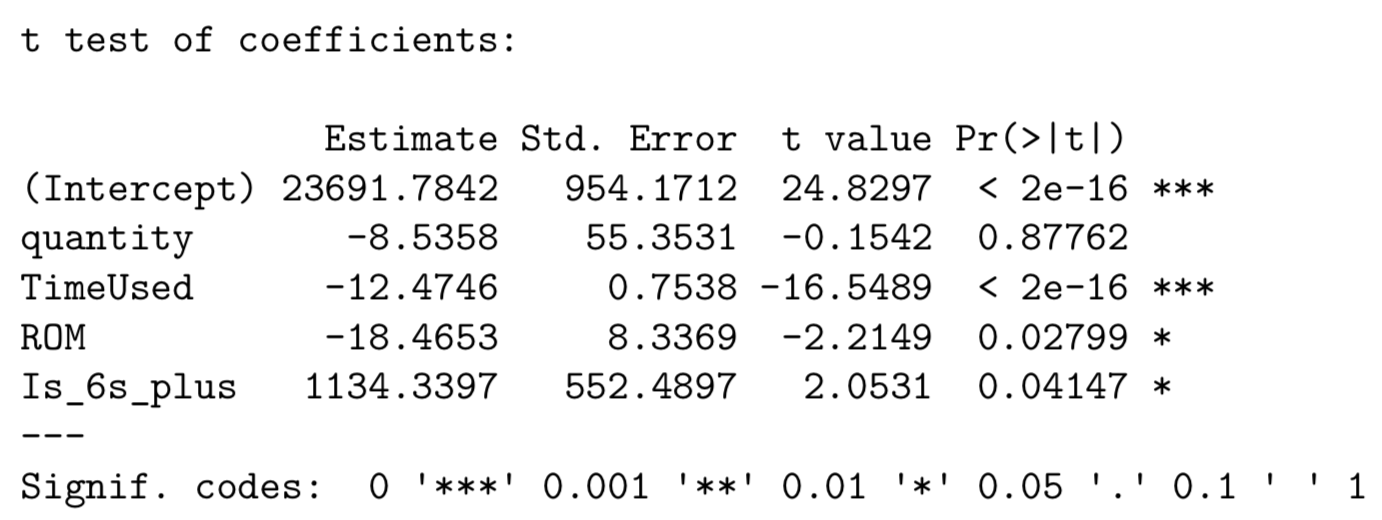
\includegraphics[width=0.8\textwidth]{figure/f05.png}
		\end{center}
	\end{figure}

\end{frame}



\subsection{Estimating the Demand Curve via IV Regression}

%%%
\begin{frame}[fragile]{Definition}

Recall the Introduction to Econometrics class:
	\begin{itemize}
		\item Quantity and Price are determined simultaneously in a system
		\item $q$ and $p$ are endogenous variables in this system
		\item OLS fails without identification
	\end{itemize}

\end{frame}


%%%
\begin{frame}[fragile]{Definition}

Take supply function estimation for example:

Supply side:
$$Q=\beta_1 P+\varepsilon$$
Demand side:
$$Q=\alpha_1 P+\alpha_2Income+u$$

where $Income$ is an exogenous variable (determined outside the system).

\end{frame}


%%%
\begin{frame}[fragile]{Definition}

We cannot estimate $\beta_1$ for the supply function via estimating the following regression model with OLS:

$$Q=\beta_1 P+\varepsilon$$

Why? Because of Endogeneity!

We need to find the demand shifter! $\rightarrow$ $Income$

\end{frame}


%%%
\begin{frame}[fragile]{Definition}

	\begin{figure}
		\begin{center}
			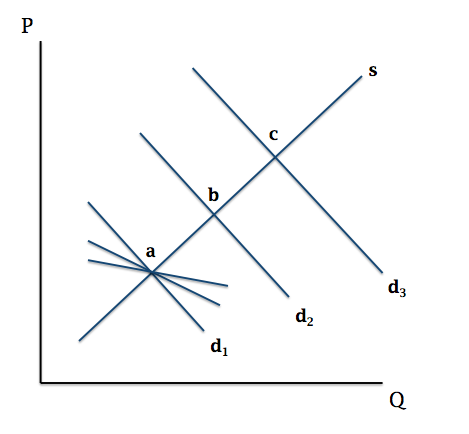
\includegraphics[width=0.6\textwidth]{figure/f06.png}
		\end{center}
	\end{figure}

\end{frame}


%%%
\begin{frame}[fragile]{Definition}

A demand shifter only affects the quantity demanded, and do no effects on quantity supplied.

Similarly, as long as we want to find the demand curve, we need to find a supply shifter.

A supply shifter is simply an IV (Instrument Variable)

\end{frame}

%%%
\begin{frame}[fragile]{IV: TSMC or Samsung?}

我們 propose 一個 IV,它是「販賣或購買 iPhone 6s 的貼文內是否標注了『台積電/TSMC 晶片』或『三星/Samsung 晶片』」, 因此我們的 IV 為兩個 Dummy Variable,分別以 $IsTSMC$ 及 $IsSamsung$ 稱之

由於 2015.9.25 發表 iPhone 6s 及 6s Plus 之後,隨即發生了「晶片門」事件

\end{frame}

%%%
\begin{frame}[fragile]{IV: TSMC or Samsung?}

我們真實想估計的 demand function(非 inverse demand function)是

$$q_t^d = \beta_0 + \beta_1 p_t + \beta_3 W_t + \varepsilon_t$$

where $W_t$表示其他外生變數。但由於$p_t$存在內生性問題$Cov(p_t, \varepsilon_t)\neq0$,因此我們可以透過 $IsTSMC$ 以及 $IsSamsung$ 此二外生變數來 serve $p_t$

\end{frame}


%%%
\begin{frame}[fragile]{IV: TSMC or Samsung?}

	\begin{figure}
		\begin{center}
			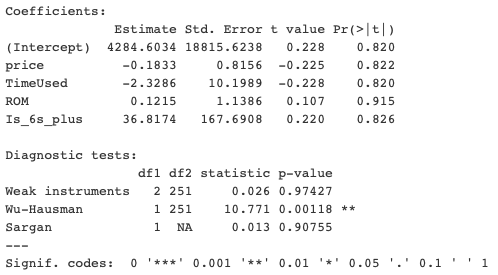
\includegraphics[width=0.8\textwidth]{figure/f07.png}
		\end{center}
	\end{figure}

\end{frame}


%%%
\begin{frame}[fragile]{IV Regression}

也就是demand function是:
$$q^d = 4284.60 - 0.18328 p$$

移項得到inverse demand function:
$$p = 23377.34 -5.4561 q^d$$

Recall the WTP estimated:
$$p = 23691.78 -8.64 q^d$$

IV Estimation 所給我們的估計較為保守
\end{frame}


\subsection{The probability of successfully selling an iPhone 6s}

%%%
\begin{frame}[fragile]{Binary Response Model}

	\begin{figure}
		\begin{center}
			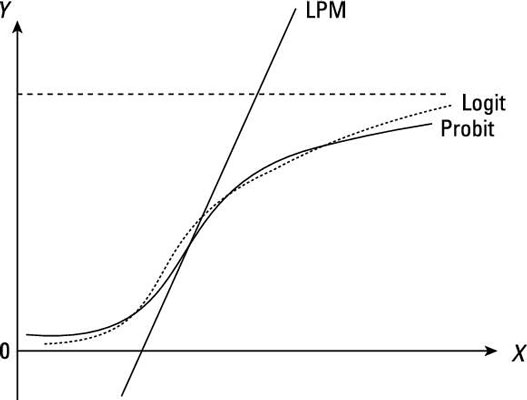
\includegraphics[width=0.8\textwidth]{figure/f08.png}
		\end{center}
	\end{figure}

\end{frame}


%%%
\begin{frame}[fragile]{Binary Response Model}

以「是否賣出」為被解釋變數

$$IsSold = \beta_0 + \beta_1 price + \beta_2 ROM + \beta_3 i6sPlus+ \beta_4 TimeUsed+ \beta_5 D_{female}+ \beta_6 color $$

\end{frame}


%%%
\begin{frame}[fragile]{Binary Response Model : LPM}

	\begin{figure}
		\begin{center}
			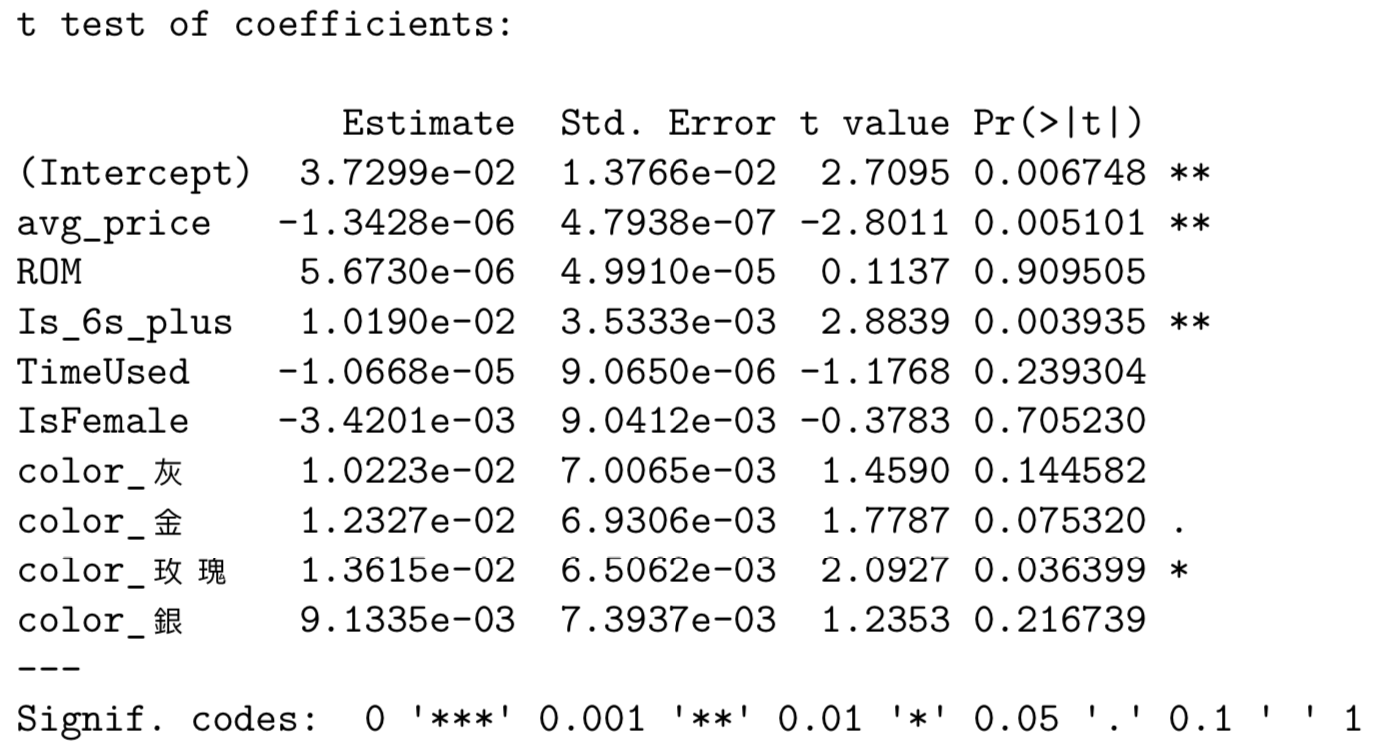
\includegraphics[width=0.8\textwidth]{figure/f09.png}
		\end{center}
	\end{figure}

\end{frame}

%%%
\begin{frame}[fragile]{Binary Response Model : Probit}

	\begin{figure}
		\begin{center}
			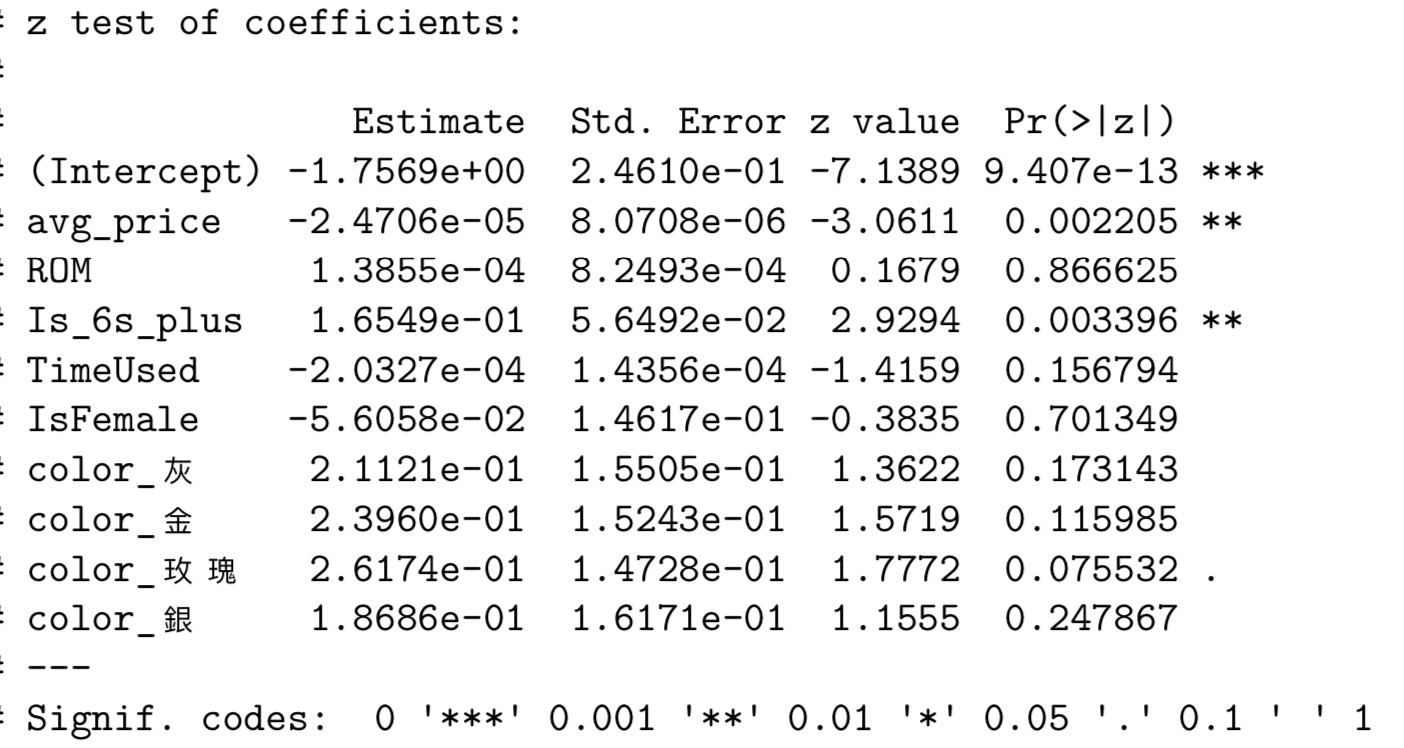
\includegraphics[width=0.8\textwidth]{figure/f10.png}
		\end{center}
	\end{figure}

\end{frame}

%%%
\begin{frame}[fragile]{Binary Response Model : Logit}

	\begin{figure}
		\begin{center}
			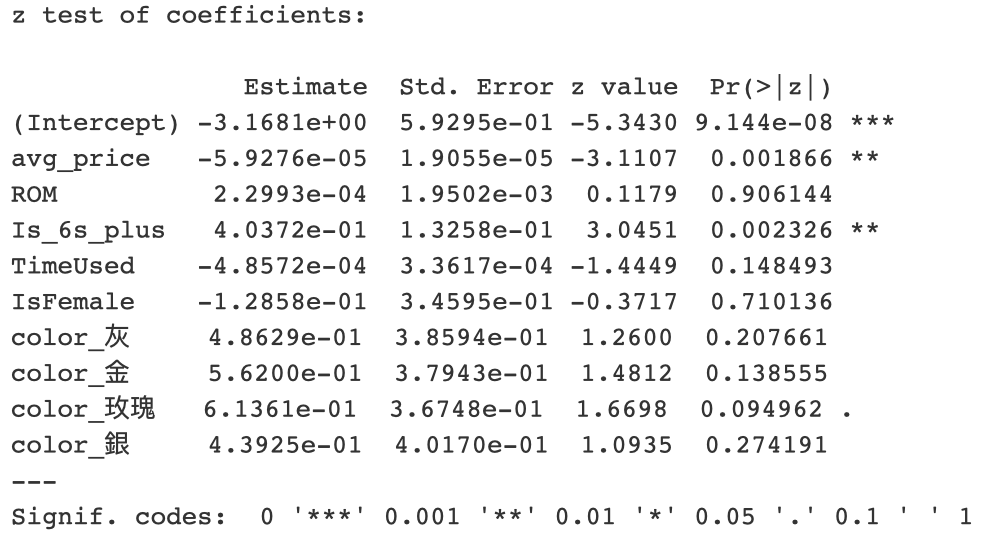
\includegraphics[width=0.8\textwidth]{figure/f11.png}
		\end{center}
	\end{figure}

\end{frame}


%%%
\begin{frame}[fragile]{Binary Response Model}

\begin{itemize}
	\item 最重要的因素仍是價格:價格越低,成交的機率就越高
	\item 「玫瑰金」在2015 年推出 iPhone 6s 時是新出的顏色
\end{itemize}

\end{frame}



\end{document}